\documentclass{paper}
\usepackage{times}
\usepackage{geometry}
\geometry{letterpaper, portrait, margin=1in}
\usepackage[utf8]{inputenc}
\usepackage{enumitem,amssymb}
\usepackage{ragged2e}
\usepackage{physics}

\usepackage{caption}
\usepackage{hyperref,url}

\usepackage{graphicx}
\usepackage{epstopdf}
\usepackage{tikz}
\graphicspath{{data/cos-w2}}

\usepackage{biblatex}
\bibliography{refs} %refs.bib

\title{cos-w2 questions}
\author{ariahayd}
\date{8 February 2022}

\begin{document} 

% set frameboxes to be borderless
\setlength{\fboxsep}{0pt}
\setlength{\fboxrule}{0pt}

\maketitle

\begin{enumerate}
    \item % 1. 
      \begin{enumerate}
        \item
          Gavitational mass is the property of an object that affects the
          local gravitional field. This mass is the active mass in a mass-mass
          interaction in the Newtonian model.
        \item
          Inertial mass is separate property of an object the responds to
          the local gravitational field. The inertial mass is passive, or 
          responsive, in the Newtonian forces model between two mass in a 
          gravitational interaction. The inertial mass acts to dampen the
          acceleration of an object in a gravitional field.
      \end{enumerate}

      There are objections to the simple model for two-body interactions
      under Newtonian gravity:
      \begin{enumerate}
        \item
          Observationally, the elliptical orbit of Mercury was seen to
          precess: the semi-major axis rotated over many orbits. This meant
          that some component of the inertial frame containing the 
          Mercury-Sun system was rotating and that the Mercury is not a simple 
          two-body interaction about the center of mass of the Sun and planet.
        \item
          Candidate absolute inertial frames (a frame on the surface of the
          Earth, a between bodies in the Solar System, etc.) are all rotating
          in orbits among larger systems, which average to the Newtonian 
          inertial frame, but contribute accelerations to the systems. 
      \end{enumerate}
      
      The Newtonian model for gravity is consistent for inertial frames, local
      areas for interactions without any component of acceleration from 
      outside of the frame. Frames must be non-accelerating relative to 
      each other for Newtonian interactions. Mach's Principle is
      the generalization that Newton's Laws are valid for inertial frames 
      relative to each other rather than to a static background of no 
      acceleration in empty space.


    \item % 2. 
      For the photon \(\nu\) in Figure \ref{fig:field} with energy 
      \(E = h \nu\), the change in energy across the gravitational potential 
      is \(E=-U\) within the potential well and \(E=-(U+\Delta{U})\) as the 
      photon climbs the potential. Because of conservation of energy, the 
      energy of the photon becomes \(E= h \Delta{\nu}\) as it traverses the 
      potential, where \(\Delta{\nu} \propto \Delta{U}\).

      \begin{figure}[!htb]
        \begin{center}
          \fbox{ 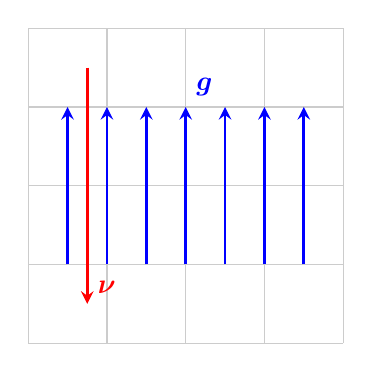
\begin{tikzpicture}
            \draw[thin,gray!40] (-2,-2) grid (2,2);
            \draw[line width=1pt,blue,-stealth](-1.5,-1)--(-1.5,1);
            \draw[line width=1pt,red,-stealth](-1.25,1.5)--(-1.25,-1.5) 
              node[anchor=south west]{\(\boldsymbol{\nu}\)};
            \draw[line width=1pt,blue,-stealth](-1,-1)--(-1,1);
            \draw[line width=1pt,blue,-stealth](-0.5,-1)--(-0.5,1);
            \draw[line width=1pt,blue,-stealth](0,-1)--(0,1)
              node[anchor=south west]{\(\boldsymbol{g}\)};
            \draw[line width=1pt,blue,-stealth](0.5,-1)--(0.5,1) ;
            \draw[line width=1pt,blue,-stealth](1,-1)--(1,1) ;
            \draw[line width=1pt,blue,-stealth](1.5,-1)--(1.5,1) ;
          \end{tikzpicture} }
        \end{center}

        \caption{Photon \(\nu\) moving through a uniform gravitation 
          field \(g\)}
        \label{fig:field}
      \end{figure}

    \item % 3.
      Space can be curved in cases where the most direct path between two
      points, the geodesic, follows a curve rather than a straight line. The
      curve can be any surve, but where the assumptions of homogeneity and
      isotropy are made, the curvature is simplified to be one of uniform
      spherical or hyperbolic curvature, or flat. A spherical curvature has
      a positive curve, which would increase the value of a geodesic compared
      to flat space, and can cause distant objects to appear larger and dimmer
      than they would would in flat space because of the elongated path of
      light following the geodesic. Hyperbolic geometry would decrease the 
      length of a geodesic compared with flatness and would cause distant
      objects to appear smaller than they would in flat space.

   \item % 4.
     For a measured radius \(a\) across a spherical surface of radius \(R\),
     the geometry is drawn in Figure \ref{fig:sphere}. The flattened radius
     is periodic with \(sin \left(\frac{R}{a}\right)\). Demonstrate 
     (\ref{eqn:curvature}) simplifies to \(k = 1/R^2\) where 
     \(C=2 \pi R sin \left(\frac{a}{R}\right)\).

     \begin{equation}
       k = \frac{3}{\pi} \lim_{a \to 0} \left( \frac{2 \pi a - C}{a^3} \right)
       \label{eqn:curvature}
     \end{equation}

     \begin{figure}
        \begin{center}
          \fbox{ \begin{tikzpicture}
            % 2-sphere surface
            \draw (0,0) circle (2cm);
            % perspective-facing circumference
            \draw (-1.404,1.404) arc (180:360:1.404 and 0.2);
            % perspective-hidden circumference
            \draw[dashed] (-1.404,1.404) arc (0:180:-1.404 and 0.2);
            % measured radius
            \draw (0,2) arc (300:360:-.9) node[midway]{\(a\)};
            % flattened radius
            \draw[dashed] (0,1.404) -- node{\tiny \(R sin 
              \left(\frac{a}{R}\right)\)}(1.404,1.404);
            % sphere radius points
            \fill[fill=black] (0,0) circle (1pt);
            \fill[fill=black] (0,2) circle (1pt);
            \fill[fill=black] (1.414,1.414) circle (1pt);
            % projection of triangle
            \draw[dashed] (0,0) -- (0,2);
            \draw[dashed] (.702,0) (0:60);
            \draw[dashed] (0,0) -- node[below]{\(R\)} (1.414,1.414);
          \end{tikzpicture} }
        \end{center}

        \caption{2-sphere of radius \(R\) on which a circle of radius \(a\) 
          will be measured to have radius \(a\), which has a flattened radius 
          of \(R sin \left( \frac{a}{R} \right) \neq a\)}
        \label{fig:sphere}
     \end{figure}

     Substitute \(C\):
       \[ k = \frac{3}{\pi} \lim_{a \to 0} \left( \frac{2 \pi a - 
         2 \pi R sin \left(\frac{a}{R}\right)}{a^3} \right) \]

     Expand \(sin \left(\frac{a}{R}\right)\) with the Maclaurin series:
       \[ sin \left(\frac{a}{R}\right) = \left( \frac{a}{R} 
         - \frac{a^3}{R^3 3!} + \frac{a^5}{R^5 5!} \right) \]

     Gives:
      \[ k = \frac{3}{\pi} \lim_{a \to 0} \left( \frac{2 \pi a}{a^3} - 
        \frac{2 \pi R}{a^3}\ \left( \frac{a}{R} - \frac{a^3}{R^3 3!} +
        \frac{a^5}{R^5 5!} \ldots \right) \right)\]

     Which simplifies under the limit \(a \to 0\):
      \[ k = \frac{3}{\pi} \lim_{a \to 0} \left( \frac{2 \pi a}{a^3} - 
        \frac{2 \pi a}{a^3} + \frac{2 \pi }{R^2 3!} - 
        \frac{2 \pi R a^5}{a^3 R^5 5!} \ldots \right) 
        = \frac{3}{\pi} \frac{2 \pi}{R^2 3!} \lim_{a \to 0}
        \left( > |a^2| \right) = \frac{1}{R^2} \]

   \item % 5.
     Because of the assumption of universal isotropy, there can be no angular
     dependence in the function \(f{(r,\theta,\phi)}\) that modifies the 
     geodesic of the fundamental geometry of space, and so simplifies to 
     \(f{(r)}\).

     Assuming homogeneity in the mass density of the universe, and with the 
     premise of general relativity that curvature is due to the mass 
     distribution, the radius of curvature cofactor \(k\) must be constant 
     in \(r\), and \(f{(r)}\) can be written as:
     \[ \frac{1}{f^2} \frac{\dd{f}}{\dd{r}} = 2 k r \]

     Separating the variables and integrating gives:
     \[ \int \frac{1}{f^2} \,df = \int 2 k r \, dr  \implies 
       - f^{-1} = k r^2 + \mathcal{C} \]

     This can be inverted to give the curvature of the geodesic as a function
     of \(r\):
     \begin{equation}
       f{(r)} = - \frac{1}{k r^2 + \mathcal{C}}
       \label{eqn:f_r}
     \end{equation}

     \(k\) relates to the geometry as the scalar factor that determines the
     degree of openess or closedness over \(\left( -\infty ,+\infty \right)\)
     where \( k = 0 \) is flat space, \( k < 0 \) is closed spherical, and
     \( k > 0 \) is open hyperbolic.

\end{enumerate}

This paper is available publicly.\cite{Hayden_Cosmology_Source_Repo}

\pagebreak
\printbibliography

\end{document}

